\famichapter{System Analysis}{This chapter analyses the FamiPet system: the data
flow between client, API, and database, and the technology stack with the
responsibility of each component.}{ch:analysis}

\section{Data-Flow Analysis}

Figure~\ref{fig:dataflow} shows the top-level data flows of the system. The
bounded system is the FamiPet backend API. Every data-producing process in the
application follows the same verified path: the client sends an HTTP request to
a route, middleware authenticates the caller, a controller validates the request
and applies ownership rules, the Mongoose model persists or reads a document in
MongoDB, and the API returns a JSON response to the client.

\begin{figure}[htbp]
    \centering
    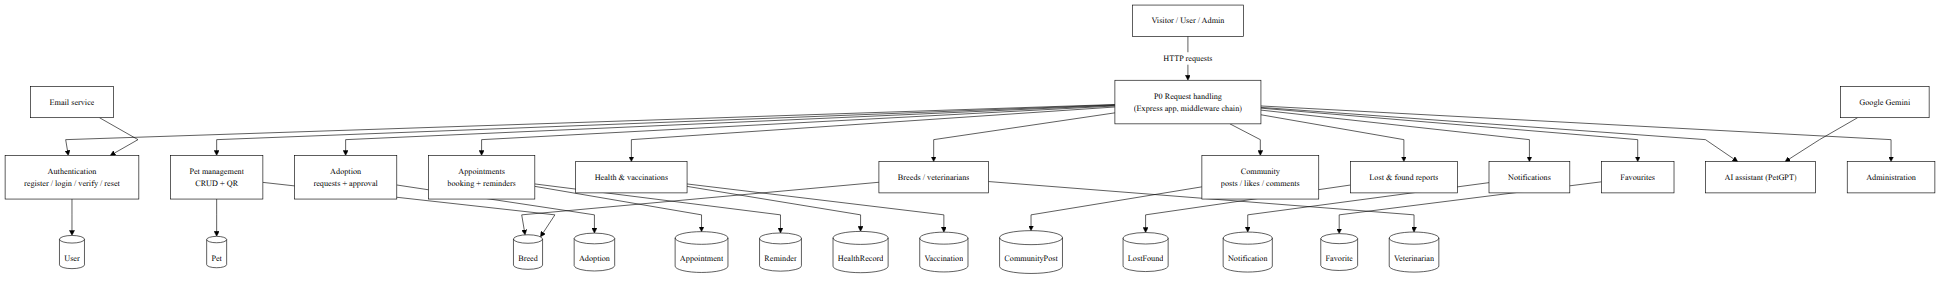
\includegraphics[width=\textwidth]{figures/03-dataflow.png}
    \caption{Top-level data-flow diagram of the FamiPet backend.}
    \label{fig:dataflow}
\end{figure}

The data-flow diagram groups the processes by the route modules that expose them
and shows the single store, MongoDB, with which every process interacts. Two
external data sinks are visible: the e-mail service, written to only by the
authentication process, and the AI service, which is reached by the AI process
and the Google Gemini endpoint.

In practice each subsystem respects the same flow, e.g. an appointment booking
produces a request on \texttt{POST /api/appointments}, and the controller writes
an \texttt{Appointment} document, synchronously creates a \texttt{Notification}
document and a \texttt{Reminder} document, and then responds with the created
record. This flow is the reason the application requires no background workers:
all derived records (notifications, reminders) are created at request time, in
the same transaction context provided by the database connection.

\section{Technology Stack}

The table below lists the technologies verified in the project implementation and
how each is used.

\begin{center}
\begin{longtable}{@{}p{3.4cm}p{3.0cm}p{8.1cm}@{}}
\toprule
\textbf{Technology} & \textbf{Type} & \textbf{How it is used} \\
\midrule
Node.js & Runtime & Executes the backend (\texttt{server.js}) on a single
process, port 5000 by default. \\
Express 4 & Web framework & Routing, JSON bodies (50\,MB limit), static files,
URL-encoded bodies, final error and 404 handlers. \\
MongoDB & Database & Persistent document store (\texttt{animal\_planet} by
default). \\
Mongoose 8 & ODM & 13 models mapped to collections; schema validation, enum
constraints, unique compound indexes, pre-save hashing hooks, query methods. \\
jsonwebtoken & Auth & Signs and verifies the bearer JWT with a 30-day expiry by
default. \\
bcryptjs & Auth & Hashes passwords with cost factor 12 and compares them on
login. \\
crypto & Auth & Generates 32-byte random tokens, hashed with SHA-256 before
storage, for e-mail verification and password reset. \\
nodemailer & E-mail & Sends HTML e-mails through SMTP (Gmail service by default). \\
multer & Upload & Accepts image uploads (JPEG/PNG/WebP, max 5\,MB) to the
\texttt{uploads/} directory. \\
qrcode & QR & Generates a PNG data-URL QR code for the digital pet identity. \\
cloudinary & Images & Optional image-hosting integration read from environment
configuration. \\
@google/generative-ai & AI & Defines the Gemini model, but the implementation
calls the REST endpoint directly with \texttt{fetch}. \\
morgan & HTTP logging & Development request logging. \\
compression & HTTP & GZIP-style response compression. \\
helmet & Security & Sets security HTTP headers, with
cross-origin-resource policy relaxed so uploaded images render on the frontend
origin (Section~\ref{sec:security}). \\
cors & Security & Origin-guard that permits the configured client origin,
localhost, and private LAN ranges. \\
node-cron & Declared & Declared but unused; no scheduled jobs exist. \\
socket.io & Declared & Declared but unused; no real-time channel exists. \\
React + TypeScript & Frontend & The in-progress migration stack used by
\texttt{frontend-react}. \\
Vite + Tailwind CSS & Frontend tooling & Build tooling and styling for the React
migration. \\
\bottomrule
\end{longtable}
\end{center}

\section{Analysis of Design Decision Consequences}

Two configuration observations are worth recording because they affect how the
system behaves at runtime.

First, the PetGPT assistant is implemented against Google's Gemini REST endpoint
(system instruction, contents, 25-second timeout, and a keyword fallback). The
OpenAI \texttt{PETGPT\_OPENAI\_*} variables in \texttt{backend/.env.example} are
not implemented, so the active provider is always Google when a key is present.
Second, reminders are not pushed asynchronously: the \texttt{Reminder}
collection records date and time, but no background scheduler delivers
notifications; the reminders are presented to the user through the reminders
API. Both facts are documented here so the reader does not mistake declared
dependencies for delivered behaviour.